\documentclass[twoside,english]{uiofysmaster/uiofysmaster}

\usepackage[toc,titletoc,title,page]{appendix} %to add appendices (and have them in toc)
\usepackage[utf8]{inputenc}
%\usepackage{mhchem} %latex chemistry symbols
\usepackage{blindtext} %to fill in dummy text
%\usepackage{cite} %to have multiple citations in one \cite{key1,key2,..} -do not use with natbib!!
\usepackage{tcolorbox} %to have boxes w color around text and math mode
\usepackage{enumitem} %to reduce vertical spacing in enumerate
\usepackage{tabu} % to set tables to page width
%\usepackage{aas_macros}

\usepackage[sort&compress,square,comma,numbers]{natbib} %to use \citet, now mixed with [nr]
\usepackage[nottoc]{tocbibind}

\usepackage{float} 
\usepackage{pdfpages}

\interfootnotelinepenalty=10000 % to force footnotes to NOT run over to the next page

%---
% to reduce space around table of contents (to fit everything into one page): 
\usepackage{tocloft}
\setlength{\cftbeforetoctitleskip}{0pt}
\setlength{\cftaftertoctitleskip}{0pt}
%---

\usepackage{epigraph}
\setlength\epigraphwidth{11cm}
\setlength\epigraphrule{0pt}

%---
\newcommand{\Sm}{$^{140}$Sm} % making it faster to write Sm140
\newcommand{\Pb}{$^{208}$Pb} 
\newcommand{\bd}{$\beta$-decay} % making it faster to write 
\newcommand{\ga}{$\gamma$}

%---
% modifying color in code listings and some style
%\usepackage{color}

% The predefined color names are: 
% black, blue, brown, cyan, darkgray, gray, green, lightgray, lime, magenta, olive, orange, pink, purple, red, teal, violet, white, yellow.
 
%\definecolor{codegreen}{rgb}{0,0.6,0} % too flashy
\definecolor{codegreen}{rgb}{0.0, 0.42, 0.24} % less flashy so comments not take all attention
\definecolor{codegray}{rgb}{0.5,0.5,0.5}
\definecolor{codepurple}{rgb}{0.58,0,0.82}
%\definecolor{codepurple}{rgb}{1.0, 0.0, 0.22} %carminered, could try it 
%\definecolor{backcolour}{rgb}{0.95,0.95,0.92} % original suggestion
\definecolor{backcolour}{rgb}{0.94, 0.97, 1.0}% aliceblue, not so flashy and not as ugly
\definecolor{LightGray}{gray}{0.95}
 
\lstdefinestyle{mystyle}{
    backgroundcolor=\color{backcolour},   
    commentstyle=\color{codegreen},
    %commentstyle=\color{codegray},    
    keywordstyle=\color{magenta},
    numberstyle=\tiny\color{codegray},
    stringstyle=\color{codepurple},
    basicstyle=\footnotesize,
    breakatwhitespace=false,         
    breaklines=true,                 
    captionpos=b,                    
    keepspaces=true,                 
    %numbers=left,     %removing line numbers in the code snippets               
    %numbersep=5pt,                  
    showspaces=false,                
    showstringspaces=false,
    showtabs=false,                  
    tabsize=2,
    %float=tp,
    %floatplacement=tbp
}
 
\lstset{
	style=mystyle,
	literate={~} {$\sim$}{1}
}
\renewcommand{\lstlistingname}{Code}
%---

%---
% new tcolorbox environment
% #1: tcolorbox options
% #2: color
% #3: box title
\newtcolorbox{mybox}[3][]
{
  colframe = #2!25,
  colback  = #2!10,
  coltitle = #2!20!black,  
  title    = #3,
  #1,
}

%---


%\bibliography{references}

\author{Trond Wiggo Johansen}
\title{I did something cool at CERN - ISOLDE
}
\date{May 2019}
 
% ----------------------------------------------------------------------------------------------------------------------
% ----------------------------------------------------------------------------------------------------------------------
%Equations
%
%The command \eqref{} works exactly like \ref{}, but it adds parantheses to a plain number.
%
%Figures and tables
%
%\autoref{} is a usefull command when refering to to figures and tables. The command creates a reference with additional text corresponding to the target's type. For example, the command \autoref{fig:myfigure} would create a hyperlink to the \label{fig:myfigure} command, wherever it is. Assuming that this label is pointing to a figure, the hyperlink would contain the text "Figure 1.1", or similar.

%Two basic citation commands, \citet and \citep for textual and parenthetical citations, respectively. …
%\citet{jon90} --> Jones et al. (1990)
%\citep{jon90} --> (Jones et al., 1990)
%\citet*{jon90} --> Jones, Baker, and Williams (1990)
%\citep*{jon90} --> (Jones, Baker, and Williams, 1990)


\begin{document}

% set space around equations
\setlength{\belowdisplayskip}{12pt} \setlength{\belowdisplayshortskip}{12pt}
\setlength{\abovedisplayskip}{12pt} \setlength{\abovedisplayshortskip}{12pt}

\maketitle

%Centering the front page, see: https://github.com/ComputationalPhysics/uiofysmaster

%%% ABSTRACT
\begin{abstract}


\end{abstract}


\begin{dedication}
To my family, for all their support and encouragement!

\end{dedication}

\begin{acknowledgements}
Supervisors Andreas Görgen and Katarzyna Hady\'nska-Kl\c ek

Nuclear Physics Group

Computational Physics Group, Morten Hjorth-Jensen

CERN-ISOLDE, Liam Gaffney

Lillefy, FFU, Fysikkforeningen

My family

Morten, Alex and Astrid.

Ina, I love you.

\subsection*{Collaboration details}
The sorting and analysis code used in this thesis has been developed at CERN-ISOLDE and can be found at \url{https://github.com/Miniball/MiniballCoulexSort}

The code for theoretical predictions of energy used in the calibration was developed by Liam Gaffney who is working at ISOLDE and has to do with analysis of data from Miniball and ISS. kinsim can be found here \url{https://github.com/lpgaff/kinsim}

Some calibration code is based on the codes of Ville Virtanen and Liam Gaffney. 

Other code/scripts have been written by the author. C++ / Python.

  \vspace{1.5cm}
  
  \noindent\textit{Trond Wiggo Johansen}\\
  
  \noindent September, 2019
  
\end{acknowledgements}


\tableofcontents


% ----------------------------------------------------------------------------------------------------------------------
% ----------------------------------------------------------------------------------------------------------------------

\chapter{Introduction}
Test \cite{Clement2016}

Test 2 \cite{OCLweb}

kinsim \cite{kinsim}

The experiment has been done before, with lower energy (and another target), Malin Klintefjord. \url{http://urn.nb.no/URN:NBN:no-56121} \newline
 
 
Experiment conducted 8th - 14th of August 2017.
% ----------------------------------------------------------------------------------------------------------------------
% ----------------------------------------------------------------------------------------------------------------------

\chapter{Theory?}

Quadrupole deformation of nuclei. \newline

Shape coexistence possible for certain regions of $N$ and $Z$.

\bigskip

- triaxial shape / shape coexistence \newline
- benchmark for theoretical models \newline
- transition probabilities and quadrupole moments between several excited states are not known \newline
- fundamental research

% ----------------------------------------------------------------------------------------------------------------------
% ----------------------------------------------------------------------------------------------------------------------


\chapter{Coulomb excitation experiment} 
\textcolor{red}{Table of abbreviations and symbols?}

\begin{table}[H]
  \centering
  \caption{Acronyms and abbreviations.}
    \begin{tabular}{ll}
        \hline
        CERN & European Council for Nuclear Research \\ 
         & (in French Conseil Européen pour la Recherche Nucléaire) \\
        ISOL & Isotope Separator On Line \\
        ISOLDE & Isotope Separator On Line DEvice \\
        PSB & Proton Synchrotron Booster \\
        GPS & General Purpose Separator \\
        HRS & High Resolution Separator \\
        EBIS & Electron Beam Ion Source \\
        REXEBIS & Radioactive beam EXperiment EBIS \\
        RILIS & Resonance Ionization Laser Ion Source \\
        HIE-ISOLDE & High Intensity and Energy upgrade \\
        RIB & Radioactive Ion Beam \\
        ENSAR2 & European Nuclear Science and Applications Research - 2 \\
        Linac & Linear accelerator \\
        ADC & Analog-to-Digital Converter \\
        TDC & Time-to-Digital Converter (or time digitizer) \\
        Coulex & Coulomb excitation \\
        \hline
    \end{tabular}
    \label{tab:acro}
\end{table}


Why CoulEx? \url{https://iks32.fys.kuleuven.be/wiki/brix/images/5/58/10_20151123_Illana_BriX15_web.pdf}

\bigskip

- nucleus excited by electromagnetic interaction. \newline
- de-excitation $\rightarrow$ gamma



\textcolor{red}{---------} \newline
\textcolor{red}{Oppgavens mål:} \newline
The ISOLDE facility at CERN has been upgraded to provide higher energies and intensities for radioactive ion beams. A new experiment to study 140Sm was performed in the summer of 2017. The goal of the experiment was to measure electromagnetic transition probabilities and electric quadrupole moments for several excited states in 140Sm by measuring Coulomb excitation probabilities. A large data set was obtained using silicon detectors to determine the energies and angles of scattered particles, and germanium detectors to measure gamma rays from excited states in 140Sm. \newline

The goal of the master thesis is to analyze the data from this experiment. The required tasks include development and improvement of data analysis software to determine Coulomb excitation yields. These yields will then, in a second step, be compared to theoretical calculations and transition probabilities and quadrupole moments will be extracted using chi-square minimization procedures. \newline


\textcolor{red}{Prosjektbeskrivelse (omfang 60 studiepoeng):} \newline
The shape of an atomic nucleus is determined by a delicate interplay between macroscopic (liquid drop) properties and microscopic shell effects. Nuclei with filled proton or neutron shells (i.e. magic nuclei) are generally spherical in shape, whereas nuclei with open shells gain energy by assuming a deformed shape. Depending on the occupation of specific orbitals, the nuclear shape can change drastically by adding or removing protons or neutrons. Certain nuclei exhibit shape coexistence, i.e. the coexistence of quantum states that correspond to different shapes. Because the shape of a nucleus is so sensitive to the underlying nuclear structure and to changes of the proton and neutron numbers, the excitation energy, or the angular momentum, observables related to the nuclear shape are used as benchmarks for theoretical models. 

Nuclei in the rare earth region, and in particular the chain of samarium isotopes, exhibit a variety of shape effects. The Sm isotope with closed neutron shell at N=82, 144Sm, is spherical in shape. Adding neutrons to 144Sm changes the deformation to an elongated (prolate) quadrupole shape. The transition from spherical to prolate shape, which occurs for 152Sm at N=90, can be interpreted as a shape-phase transition. Flattened (oblate) quadrupole shapes are predicted by theory to occur below the N=82 shell closure. An earlier experiment studying 140Sm at CERN-ISOLDE found triaxial shape for this isotope, i.e. a shape where all three principal axes of the ellipsoid have different lengths. 140Sm can therefore be considered to lie at the critical point of a phase transition from spherical to deformed, and from prolate to oblate shape. \newline

\textcolor{red}{Foreløpig tittel:} \newline
Coulomb excitation of 140Sm \newline


\textcolor{red}{Metoder som tenkes benyttet:} \newline
Multi-step Coulomb excitation with radioactive beam, isotope separation on-line technique, nuclear spectroscopy, particle-gamma and particle gamma-gamma coincidence analysis, advanced chi-square minimization procedures. \newline
\textcolor{red}{---------} \newline


\section{ISOLDE at CERN}
ISOLDE is a radioactive ion beam facility at CERN in Meyrin, Switzerland. The facility can produce over 1000 different radionuclides to be used in a wide variety of experiments in nuclear physics, atomic physics, solid state physics, life sciences and fundamental interactions. Experiments have been performed at ISOLDE since 1967 and since 2001 experiments with post-accelerated radioactive ion beams (RIBs) have been conducted. \textcolor{red}{New / moved facility in 1992, to the place as we know it today.} The high intensity and energy upgrade (HIE-ISOLDE) have made it possible to deliver energies up to 10 MeV/$u$ in 2018 \cite{Borge2018}. 
 \textcolor{red}{Cite: \url{http://iopscience.iop.org/article/10.1088/1361-6471/aa990f} and \url{http://www.scholarpedia.org/article/The_ISOLDE_facility}}  


\bigskip

ISOLDE \url{http://isolde.web.cern.ch} and \url{http://isolde.web.cern.ch/sites/isolde.web.cern.ch/files/NuclPhysNew-ISOLDE_0.pdf} and \url{http://www.scholarpedia.org/article/The_ISOLDE_facility}  and \url{http://iopscience.iop.org/article/10.1088/1361-6471/aa5f03/pdf}


HIE-ISOLDE \url{http://hie-isolde-project.web.cern.ch}, technical design \url{http://cds.cern.ch/record/2635892?ln=en}, direct to doc: \url{http://cds.cern.ch/record/2635892/files/HIE-ISOLDE_TDR.pdf}


\subsection{Beam production}

ISOLDE experimental hall (\textcolor{red}{make flow chart or show overview over the hall}):
\begin{align*}
	\text{p}^+ ~(\text{from PSB}) \rightarrow~ &\text{Production target} \rightarrow \text{GPS} \rightarrow \text{RILIS} \rightarrow \text{\textcolor{red}{REXTRAP?}} \rightarrow \\
 &\text{REXEBIS} \rightarrow \text{HIE-ISOLDE} \rightarrow \text{MINIBALL}
\end{align*}

A proton beam of 1.4 GeV ($\sim 10^{18}$ protons) from the PSB comes into the ISOLDE facility and collide with a production target \textcolor{purple}{of tantalum, producing the elements in the chart of nuclides up to tantalum. The proton beam can collide in one of the two target stations, the general purpose separator (GPS) or the high resolution separator (HRS). The GPS has one bending magnet and can deliver beams of different mass simultaneously into three beam lines, while the HRS has two bending magnets with high mass resolving power and deliver the beam into the main \textcolor{teal}{(or common)} beam line. In this experiment, the GPS was used.} The fragments travels in the beam line onward to the GPS where the mass of $A = 140$ (isobar) is selected (\textcolor{red}{separated from the rest}). 

\textcolor{red}{GPS or RILIS first??}

\textcolor{red}{RILIS or REXEBIS for ionization of the atom?} 

The resonance ionization laser ion source (RILIS) uses the method of step-wise excitation and ionization of the atom. \textcolor{red}{It is a three step excitation, where the last step leads to the ionization.}  \textcolor{teal}{RILIS selects samarium with laser (element selective process, samarium $Z = 62$). RILIS is used to produce ion beams \textcolor{purple}{of the correct element}.}

\textcolor{red}{REXTRAP}. Penning trap

REXEBIS excites the nucleus in three steps ionizing the atom, which leaves the nucleus in a high charge state. 

The HIE-linac accelerates the beam through the beam line and magnets bend the beam into MINIBALL. 

\textcolor{red}{Cite: \url{https://ac.els-cdn.com/0168583X92959079/1-s2.0-0168583X92959079-main.pdf?_tid=0ccb0647-5870-48f9-ac38-df8c0077981c&acdnat=1545216224_d359ddcc40ea1f94369c85a141edba63} and \url{https://cds.cern.ch/record/2025701/files/epjconf_inpc2013_11005.pdf} and \url{http://isolde.web.cern.ch/targets-and-separators}}

\bigskip

\textcolor{red}{"The General Purpose Separator (GPS) has one bending magnet and an electrostatic switchyard allowing the simultaneous extraction of three mass separated beams." \url{http://isolde.web.cern.ch/targets-and-separators}}

\bigskip

ISOLDE GPS++ \url{https://cds.cern.ch/record/2025701/files/epjconf_inpc2013_11005.pdf}

\bigskip


\textcolor{red}{"The RILIS is a chemically selective ion source which relies on resonant excitation of atomic transitions using tunable laser radiation." \url{http://rilis.web.cern.ch}} 

\textcolor{red}{"The principal application of RILIS is the production of ion beams of elements required for ISOLDE experiments. ... laser ionization is required to be only an element-selective process"} \url{http://iopscience.iop.org/article/10.1088/1361-6471/aa78e0}

\bigskip

\autoref{fig:accelerators} shows the CERN accelerator complex \cite{CERN-AC}. ISOLDE is located beside the PSB.


\begin{figure}[t]
	\centering
	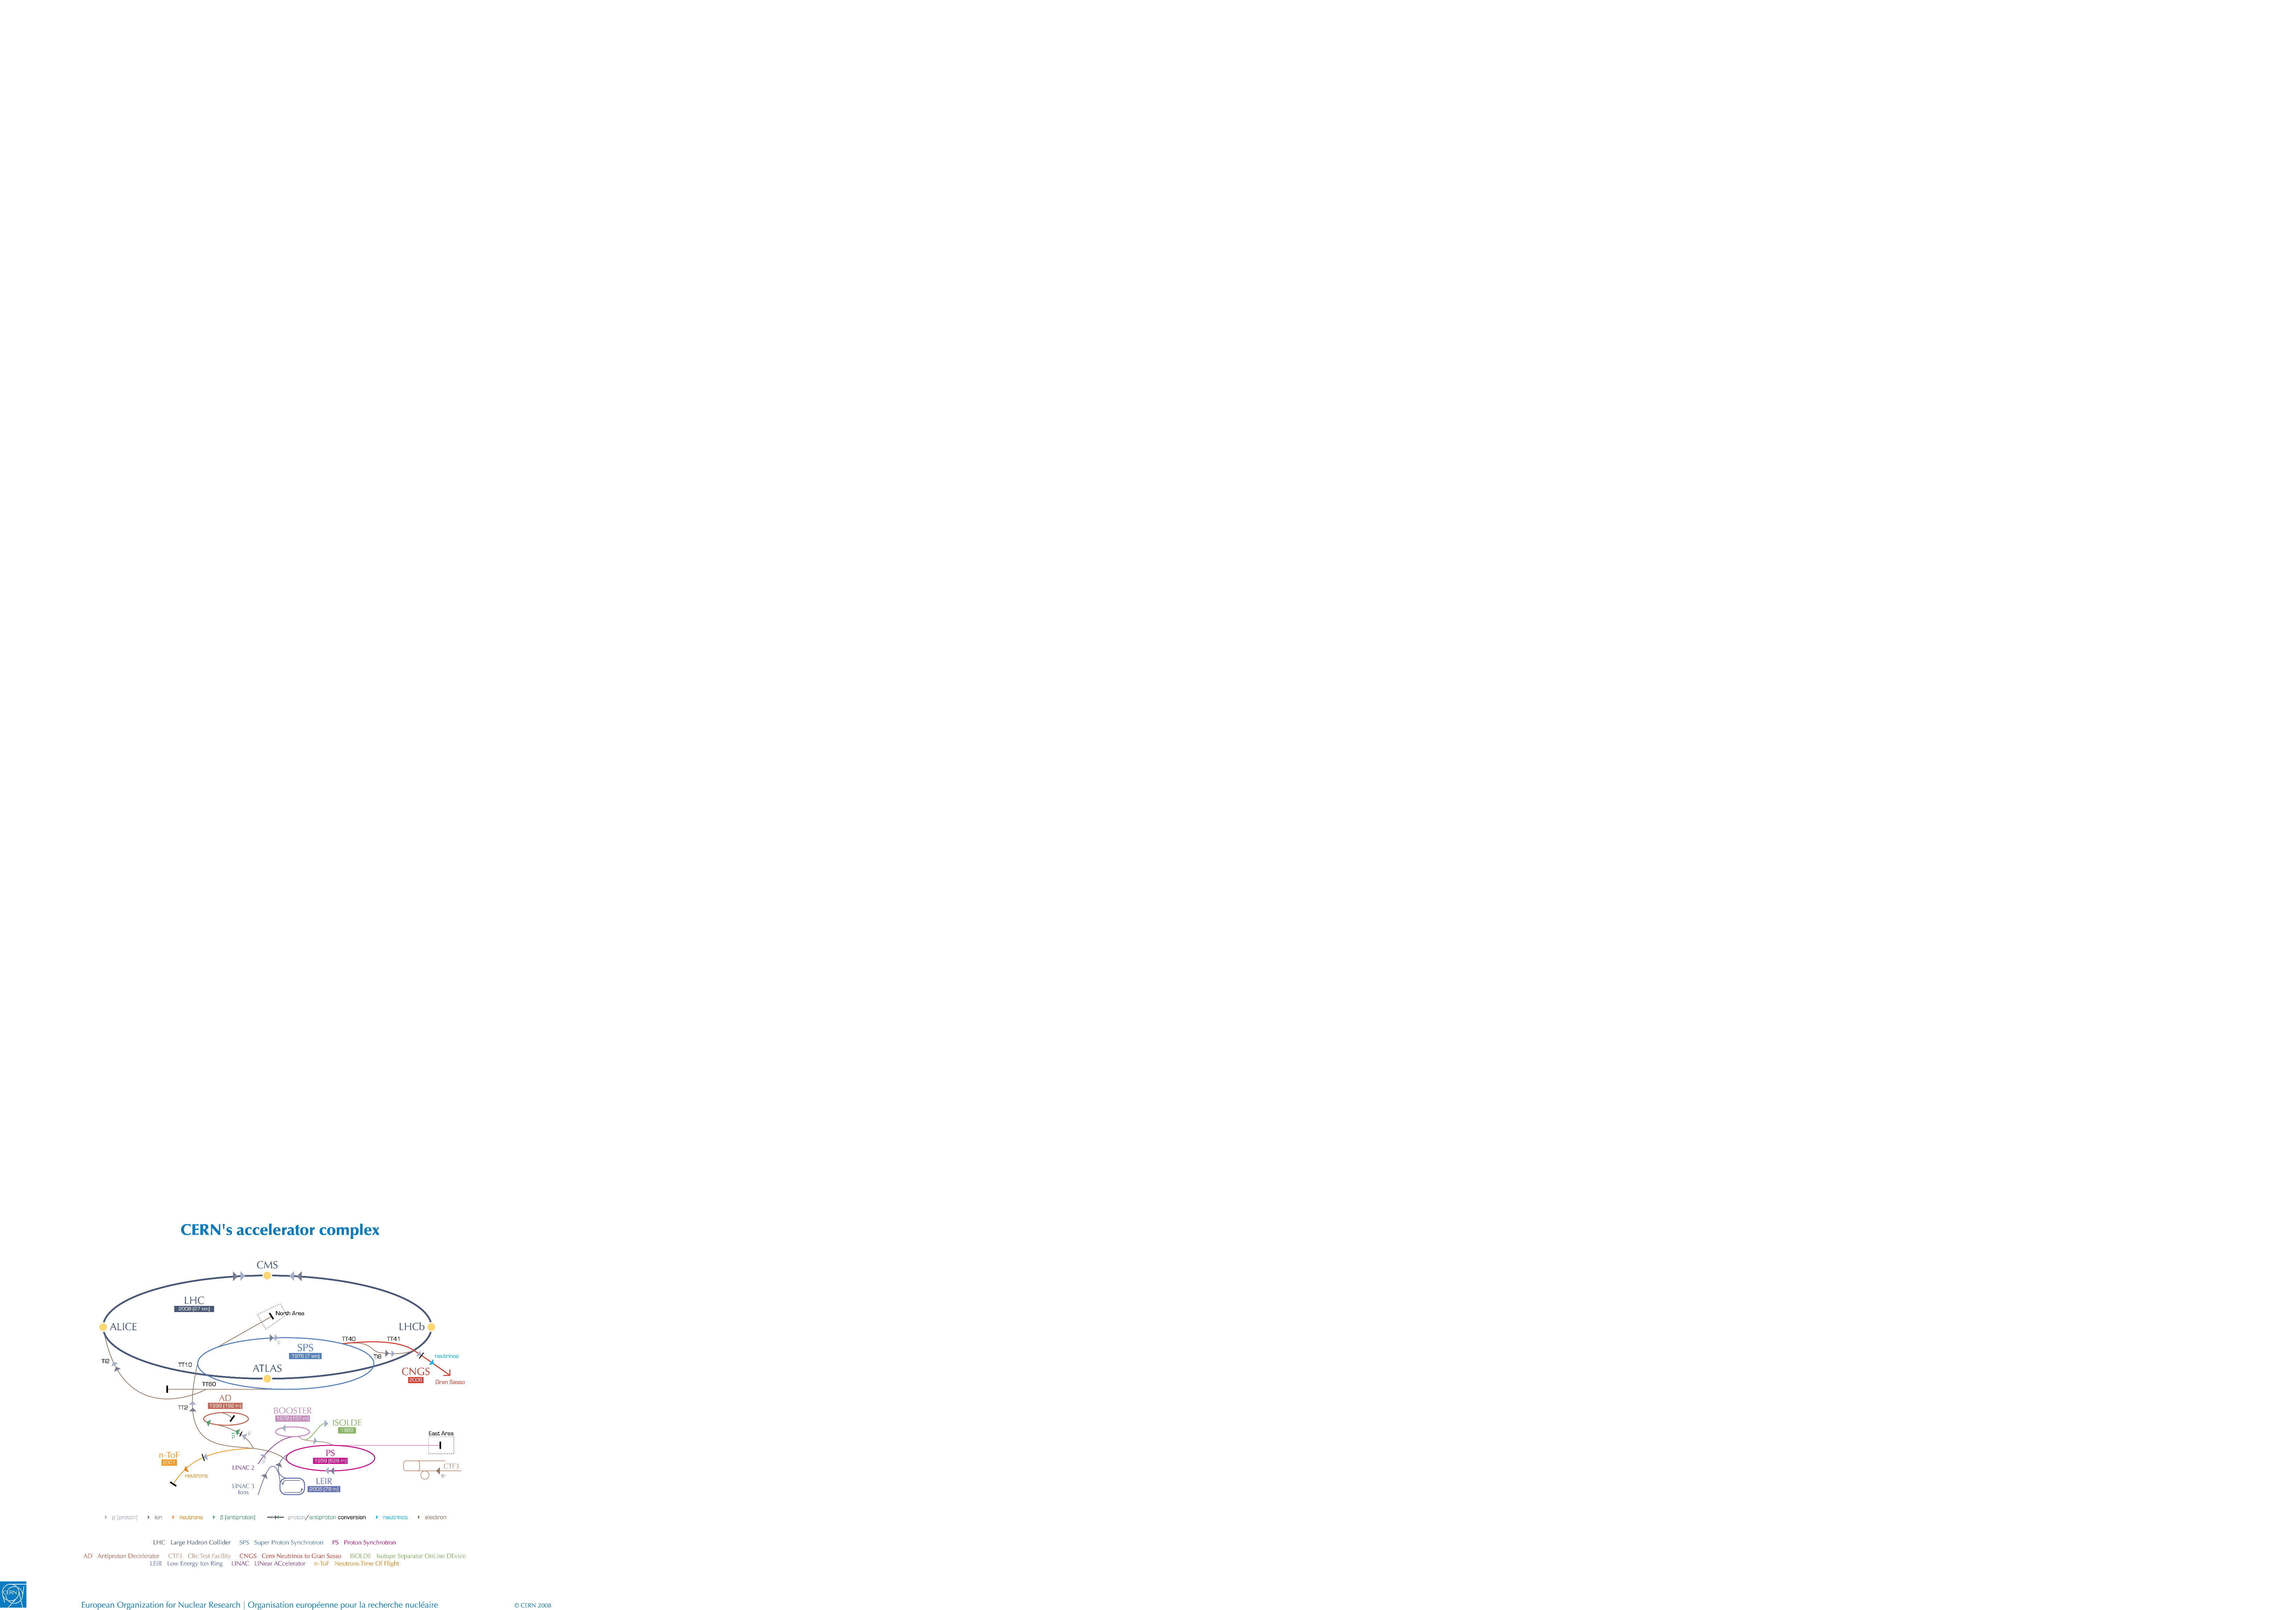
\includegraphics[width=\textwidth]{images/0812015.pdf}
	\caption{The CERN accelerator complex. ISOLDE gets accelerated protons from LINAC 2 and the PS BOOSTER.}
	\label{fig:accelerators}
\end{figure}

\bigskip

Magnets....

\bigskip

Ebis: charge breader: release beam with certain energy.


high-performance charge breeder (CB). CB based on the Electron Beam Ion Source (EBIS) technology – an EBIS Charge Breeder (ECB)


\bigskip

HIE-ISOLDE (Superconducting Linac Upgrade): Linear accelerator, HIE-linac \newline

\bigskip

Post-accelerated beams ISOLDE \url{http://iopscience.iop.org/article/10.1088/1361-6471/aa78ca}

\bigskip

ISOLDE actually uses the most protons at CERN [\textcolor{red}{ref?}].

\bigskip

Very pure beam (\textcolor{red}{did we have statistics of this?})

\bigskip

PSB \url{https://home.cern/science/accelerators/proton-synchrotron-booster}

\bigskip

REX-ISOLDE \url{http://rex-isolde.web.cern.ch}

\bigskip

RILIS \url{http://rilis.web.cern.ch} and \url{http://iopscience.iop.org/article/10.1088/1361-6471/aa78e0/meta} and \url{https://www.research.manchester.ac.uk/portal/files/60831252/FULL_TEXT.PDF} and \url{https://www.sciencedirect.com/science/article/pii/S0168583X13008914?via%3Dihub}

\bigskip

MINIBALL \url{http://isolde.web.cern.ch/experiments/miniball} and \url{https://www.miniball.york.ac.uk/wiki/Main_Page}

\bigskip

ENSAR2 \url{http://www.ensarfp7.eu}

\bigskip

Beam production \url{http://tuprints.ulb.tu-darmstadt.de/4599/1/TUDthesis_Christoph%20Seiffert.pdf}

\bigskip

Test \cite{CERN-AC}, copyright: \url{https://copyright.web.cern.ch}

\bigskip

CERN Document Server  \url{https://cds.cern.ch}


\subsection{Target}

\Pb\ was chosen as a target. Want high $Z$ so that the probability of excitation is high. Not enough beam energy to excite \Pb. \newline

Highest $Z$ for maximum excitation probability.


Contamination... finger print [\textcolor{red}{picture}]


\section{Miniball}

Pictures \url{https://cds.cern.ch/record/844871?ln=en}

\subsection{Particle detector, DSSSD (CD)}

16 rings, 12 strips effectively (24 strips, 12 pairs with two strips making a pair)

Angle coverage: [18.4$^\circ$, 56.6$^\circ$]


\subsection{\ga\ detectors, HPGe}

24 six-fold segmented. 8 clusters of 3 crystals each. Each crystal segmented in 6 parts (144 segments in total).

\bigskip

Cryo-modules

\section{Experimental setup}
\Sm ~Coulomb excitation experiment.

Experiment code: IS558 

Ta: tantalum (Z = 73)

Sm: samarium (Z = 62)

Pb: lead (Z = 82) \newline



Beam: \Sm (T$_{1/2} \approx 15$ min, 4.65 MeV/$u$, total 651 MeV), excellent purity

Target: \Pb (Thickness: 1.4 mg/cm$^2$)


Small angle: Forward scattering: Larger distance, weaker \textcolor{red}{EM}-field, less excitation probability.

Large angle: Backward scattering: Closer distance, stronger \textcolor{red}{EM}-field, higher excitation probability. \newline


\bigskip

Expect to measure transition probabilities $B(E2)$ and quadrupole moment (nuclear deformation). 

\bigskip

Level scheme (from Klintefjord?)

% ----------------------------------------------------------------------------------------------------------------------% ----------------------------------------------------------------------------------------------------------------------



\chapter{Data analysis} 

ROOT: analysere data

kinsim3 \url{https://github.com/lpgaff/kinsim} + SRIM \url{http://www.srim.org}

\bigskip


\begin{table}[H] \centering 
\caption{Computer used for data analysis}
\label{tab:PC}
\begin{tabular}{ll}
\hline
Model & MacBook Air (13-inch, 2017) \\
\hline
Processor & 1.8 GHz (Intel Core i5) \\
Memory & 8 GB (1600 MHz DDR3) \\
\hline
\end{tabular}
\end{table}

Runtime for sorting data: \newline
TreeBuilder (online calibration): $\sim$ 40-45 min \newline
AQ4Sort (online calibration): $\sim$ 120 min

\begin{table}[H] \centering 
\caption{Runtime for sorting data.}
\label{tab:PC}
\begin{tabular}{ll}
\hline
Executable & Runtime [min] \\
\hline
TreeBuilder & $\sim$ 45 \\
AQ4Sort & $\sim$ 120 \\
\hline
\end{tabular}
\end{table}

The runtime of the bash script was done with the built in script time

\begin{lstlisting}[language=sh]
$ time ./AQ4S.sh Sm online TB
...
real	45m19.265s
user	42m49.653s
sys	0m39.665s
\end{lstlisting}


\begin{lstlisting}[language=sh]
$ time ./AQ4S.sh Sm online Q4
...
real	121m40.830s
user	116m18.361s
sys	1m17.809s
\end{lstlisting}


\begin{lstlisting}[language=sh]
$ time ./AQ4S.sh Sm user TB
...
real	41m11.282s
user	39m45.592s
sys	0m27.777s
\end{lstlisting}


\begin{lstlisting}[language=sh]
$ time ./AQ4S.sh Sm user Q4
...
real	143m47.600s
user	128m6.174s
sys	1m50.921s
\end{lstlisting}


\bigskip

particle-gamma and particle-gamma-gamma coincidence

\textcolor{red}{sjekk opp om energi fra online kalibrering passer med simuleringen.}

\section{Data and sorting}
The analysis code for Miniball data is named MiniballCoulexSort and is available on GitHub at \url{https://github.com/Miniball/MiniballCoulexSort}. 
The main steps of how to download, install and use it is outlined in the README.md file in the GitHub repository. 

Data from Miniball comes in the form of .med-files (Miniball Event Data). 
In order to analyze this data in ROOT\footnote{ROOT is a data analysis framework made at CERN.} the first part of the sorting is just to convert the .med-files into .root-files with the script MedToRoot. 

To get useful information out of the converted .root-files, the Treebuilder script is used. 
The .root-file(s) and a calibration file is given to the Treebuilder so it can make event trees that can be used for analyzing the Coulomb excitation events. 

One script that is mentioned in the Miniball GitHub repository, but not showed how to use, is the AQ4Sort. It is used in the same way as the TreeBuilder script, but it sorts the histograms in another way. 
This script is used before and during the calibration of the detectors, because it gives information about every single ring and every single back strip. The one thing to note here, is that the numbering of the detector rings and strips are different from the ones used in Treebuilder. 



\section{Helping scripts}
All of my scripts are available in the GitHub repository \url{https://github.com/wiggoen/MasterThesis}.

In order to not copy and paste the sorting command in the terminal for every data file, I made two bash scripts to do this. The script \textbf{M2R.sh} is using MedToRoot to take in as many files as you want, and sort it in one go. The other script is \textbf{AQ4S.sh}, which is using either AQ4Sort or Treebuilder to sort a lot of files in one go. 

I also made other helping scripts to get histograms, do fitting, comparison and calibration. 

My scripts: MultiFit.cpp, MultiPlot.cpp, ++ (python, bash,..)


\section{Simulation}
To calibrate the data, we need to know the expected energy of the centroids of the peaks. 
This was done by simulating the experiment in a program called kinsim3. The program is written by Liam Gaffney\footnote{Liam Gaffney is a fellow at ISOLDE, affiliated with MINIBALL.} and the purpose of the program is to simulate the kinematics of the experiment. 
It takes into account the Silicon dead layer. 

kinsim3 generates pdf-files of the stopping powers automatically. 
The rest of the plots are available inside the root-file. 
To get the energy simulation for each ring, the function \textbf{cd\_sim\_plots()} from the script \textbf{MultiPlot.cpp} was used. 

\bigskip


CD to target distance: 26.98 mm.


Simulation done by kinsim3

\begin{figure}[H]\centering
    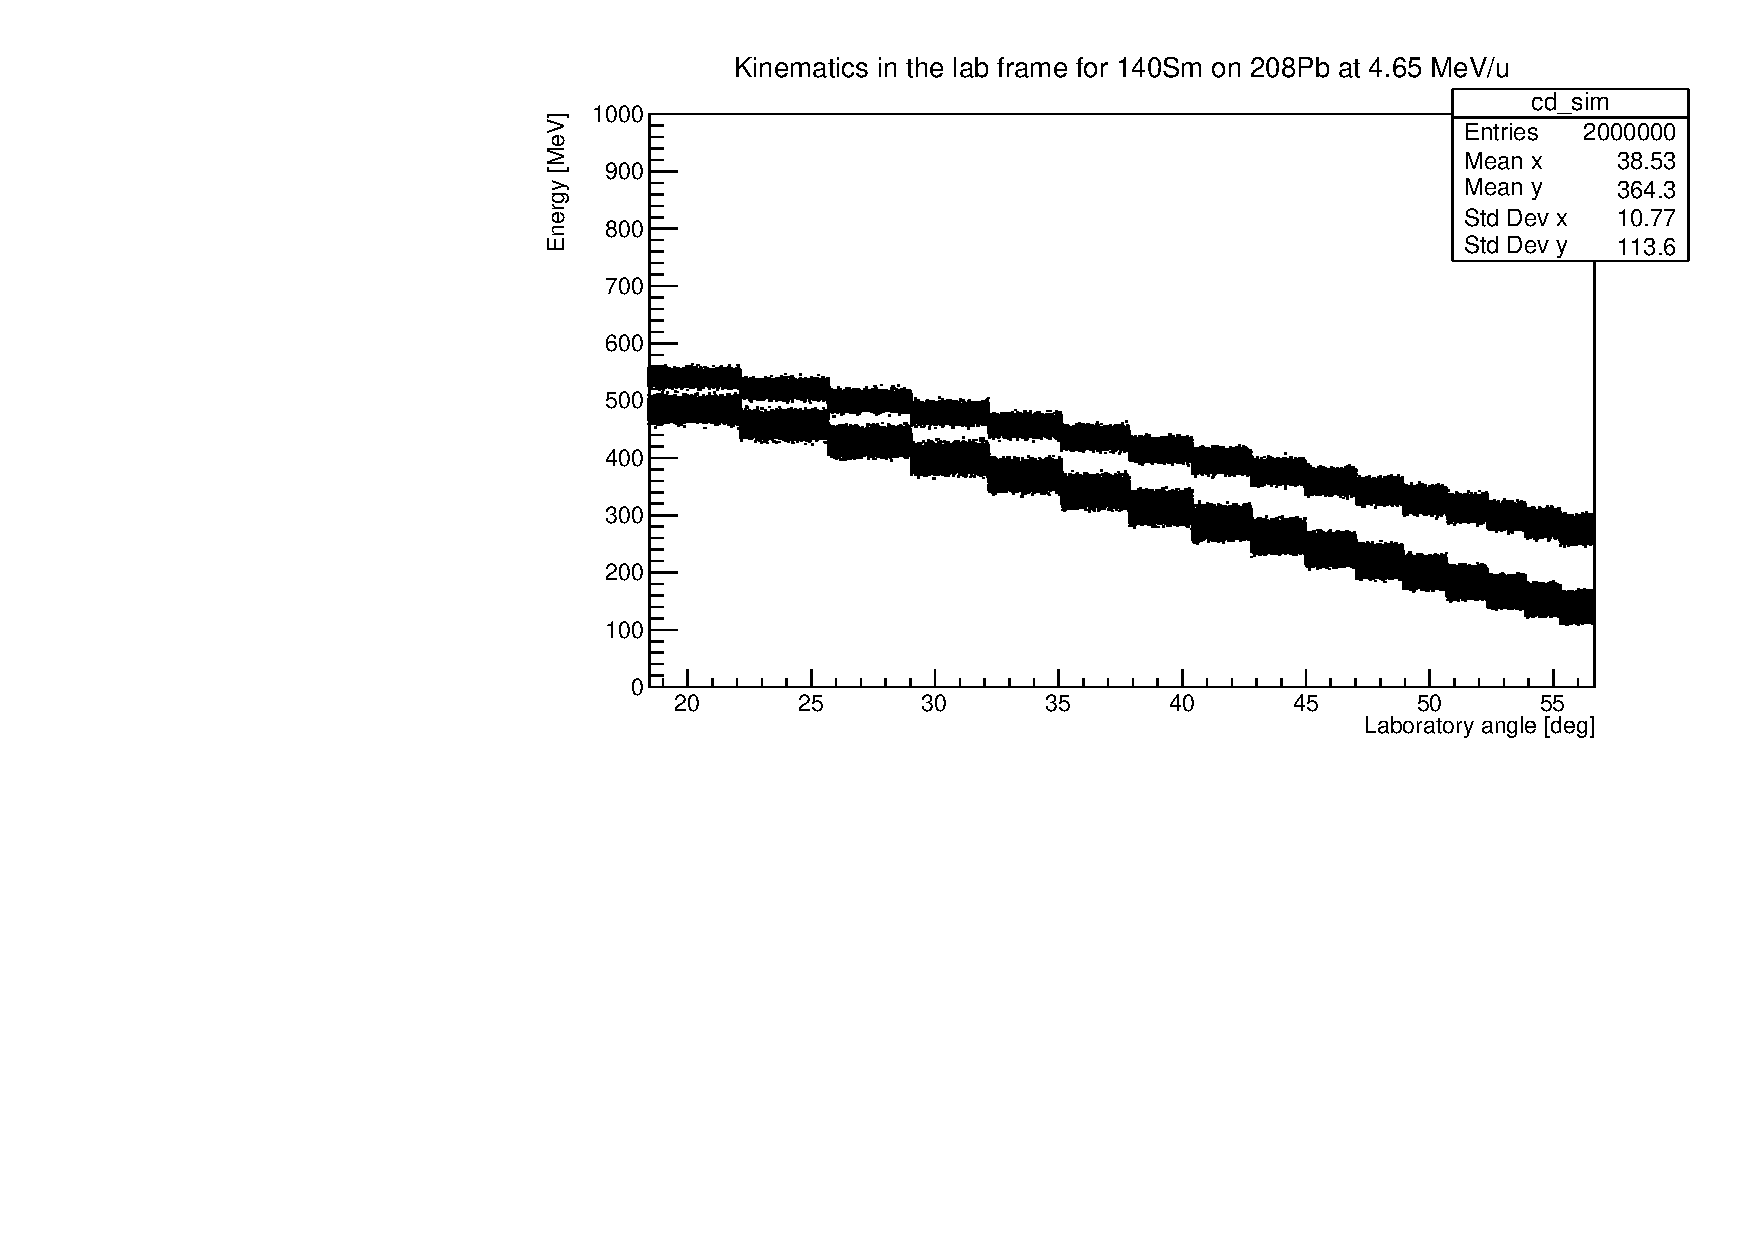
\includegraphics[width=\linewidth]{../Plots/simulation/kin_140Sm_208Pb.pdf}
\end{figure}


\textcolor{red}{Mail fra Liam:} \newline
"the source has a thickness of 1.23 mm, which needs to be factored in so that the CD to target distance is the CD to source distance PLUS the source thickness, i.e. 25.78 mm + 1.23 mm =  27.01 mm. 
This is very close to the 26.98 mm you got from us in August. 
\textcolor{red}{I think that the source data was reanalysed since the original blog entry, giving the 0.03 mm difference!}" \newline



Terminal: Simulation: 140Sm on 208Pb:
\begin{lstlisting}[language=sh]
$ cd GitHub/Miniball/kinsim
$ root
root [0] .L kinsim3.cc+
root [1] kinsim3(62, 82, 140, 208, 1.4, 4.65, 0.02, 1.0, 0.6, 27.01, false, 1e6, "../SRIM")
\end{lstlisting}


kinsim3 function:
\begin{lstlisting}[language=c++]
void kinsim3( int Zb, int Zt, double Ab, double At, double thick /* mg/cm^2 */, double Eb /* MeV/u */,
    double dEb = 0.1 /* MeV/u */, double Ex = 1.0 /* MeV */, double res = 0.6 /* % */,
	double cd_dist = 28.0 /* mm */, bool flat = false /* angular distribution? */,
	long Nevts = 1E6, string srim_dir = "../srim" )
\end{lstlisting}

\bigskip

\textcolor{red}{Say something about SRIM files.}

\bigskip



\section{Calibration}
For each file converted with MedToRoot, the program makes four files; OffBeam, OnBeam, OnBeamBackground and Scaler. The file we are interested in for analysis is the OnBeam file. 

First all of the interesting files are converted with the M2R.sh script. 
Then the OnBeam files from M2R.sh is run through using Treebuilder in the AQ4S.sh script. 
Using the MultiPlot.cpp script, the ADC time offsets can be extracted
\begin{lstlisting}[language=sh]
$ cd /Users/trondwj/GitHub/MasterThesis/Scripts/plotting
$ root
root [0] .L MultiPlot.cpp 
root [1] check_ADC_time_offsets("setup_Sm.txt", "online")
\end{lstlisting}
or they can be manually reached by
\begin{lstlisting}[language=sh]
$ cd /Users/trondwj/GitHub/MasterThesis/Sorted_data
$ root Sm_user-TreeBuilder-2019-03-22.root 
root [1] new TBrowser()
\end{lstlisting}
and in the browser, the histograms named tdiff\_gp\_i (where i is a number between 0 and 3) will lie under all the folders.


\textcolor{red}{HUSK:} Si noe om ADC time offsets. Og at man må se på det tidlig, så resortere.


M2R.sh $\rightarrow$ AQ4S.sh$\rightarrow$ check time offset $\rightarrow$ threshold $\rightarrow$ AQ4\_fit() $\rightarrow$ particle-calibration.py $\rightarrow$  ADC\_generator.py $\rightarrow$ copy the calibration from the terminal and paste into calibration file 


Simulation fit $\rightarrow$ AQ4\_fit() $\rightarrow$ particle-calibration.py $\rightarrow$  ADC\_generator.py $\rightarrow$ copy the calibration from the terminal and paste into calibration file 

Visualize plots using ROOT and the scripts. 



Skriv om scriptene som er lagd, og at det var litt vanskelig å automatisere kalibreringen. Hvis det skulle vært gjort måtte vi funnet en "left skewed function". 


I log-skala ser dette mer Gaussisk ut, men det er ikke det i non-log skala. 


Back detector calibration: There are just too much individual differences to calibrate the back detectors with a simple script given a range for all 12 back strips. I found out this way to late. There isn't any range to rule them all, at least since the fitting function can behave very strange given a too small or too big range.

\subsection{ADC time offsets}


\subsection{Threshold}
* Threshold (forskjellig i log/ikke-log skala)

Threshold: The code has a default threshold of 100, but in some cases this is too much and some cases this is not enough. So for each adc channel, the threshold can be set. We don't want to include the "pedestal". Charge sharing.
Won't cut too much or too little..

Sjekk hva Liam skrev i mailen. 

\subsection{Particle detector}
\subsubsection{Online calibration}







\subsubsection{User calibration}
ADC: Analog to digital converter (Mesytec)

TDC: Time to digital converter

DSSSD: Double-Sided Silicon Strip Detector $\implies$ CD

must remove the inner ring from data analysis because of damage

\begin{align*}
	gain = \frac{E_{Sm} - E_{Pb}}{Ch_{Sm} - Ch_{Pb}}
\end{align*}

\begin{align*}
	offset = E_{Sm} - gain \cdot Ch_{Sm}
\end{align*}
in keV.

\textcolor{red}{Hvis man har flere sentroider bruker man bare lineær regresjon. Gjelder for baksiden!}



\subsection{Gamma detectors}

DGF: Digital \ga~ finder

addback, singles, ...


\section{Doppler correction}

% ----------------------------------------------------------------------------------------------------------------------% ----------------------------------------------------------------------------------------------------------------------


\chapter{Experimental results}


% ----------------------------------------------------------------------------------------------------------------------% ----------------------------------------------------------------------------------------------------------------------


\chapter{Discussion}


% ----------------------------------------------------------------------------------------------------------------------% ----------------------------------------------------------------------------------------------------------------------

\chapter{Summary and outlook}


% ----------------------------------------------------------------------------------------------------------------------% ----------------------------------------------------------------------------------------------------------------------




% ----------------------------------------------------------------------------------------------------------------------% ----------------------------------------------------------------------------------------------------------------------

\begin{appendices}
\chapter{Connecting MiniballCoulexSort with ROOT}
To connect MiniballCoulexSort with ROOT you need them to share their libraries with each other. This is done with a dynamic loader. You can find out more here: \url{https://root.cern.ch/root/htmldoc/guides/users-guide/ROOTUsersGuide.html#file-system.rootrc}. 

You have to make a \textbf{.rootrc} file in your home folder on your computer. In the \textbf{.rootrc} file you want to write something like this 
\begin{lstlisting}[language=sh]
Unix.*.Root.DynamicPath:    .:</Users/trondwj/GitHub/ROOT-framework/build/lib>:/Users/trondwj/GitHub/Miniball/MiniballCoulexSort/lib:
\end{lstlisting}
This should all be in one line. The first part is to tell the system to use the dynamic loader of ROOT to connect the given paths that follow. In my case the lib folder of the ROOT install was at 
\begin{lstlisting}[language=sh]
/Users/trondwj/GitHub/ROOT-framework/build/lib
\end{lstlisting}
and the lib folder of the MiniballCoulexSort was at
\begin{lstlisting}[language=sh]
/Users/trondwj/GitHub/Miniball/MiniballCoulexSort/lib
\end{lstlisting}
These paths is totally individual, and you will probably not have it in the same place. Therefore these paths must be changed to fit your system. 

After making the file you either have restart the terminal or you can source the file by writing this in the terminal
\begin{lstlisting}[language=sh]
$ source ~/.rootrc
\end{lstlisting}


\chapter{Running ROOT and MiniballCoulexSort from anywhere in the terminal}
To run ROOT or the different scripts of MiniballCoulexSort anywhere in the terminal, you have to edit your \textbf{.bash\_profile} file [.bash\_profile on MacOS, .bashrc on Linux]. In my \textbf{.bash\_profile} I used this 
\begin{lstlisting}[language=sh]
# Run ROOT from anywhere
export ROOTSYS=$HOME/GitHub/ROOT-framework/build
export PATH=$ROOTSYS/lib:$PATH
export PATH=$ROOTSYS/bin:$PATH
export DYLD_LIBRARY_PATH=$ROOTSYS/lib:$DYLD_LIBRARY_PATH

# Run MiniballCoulexSort from anywhere
export DYLD_LIBRARY_PATH=$HOME/GitHub/Miniball/MiniballCoulexSort/lib:$DYLD_LIBRARY_PATH
export PATH=$HOME/GitHub/Miniball/MiniballCoulexSort/lib:$PATH
export PATH=$HOME/GitHub/Miniball/MiniballCoulexSort/bin:$PATH
\end{lstlisting}
The DYLD\_LIBRARY\_PATH is used on Mac only. On other systems, use \newline LD\_LIBRARY\_PATH. You need to locate the lib and bin folders for both ROOT and MiniballCoulexSort and change them to fit your system, and in addition you need the build folder of your ROOT install.



\chapter{Other appendicies}
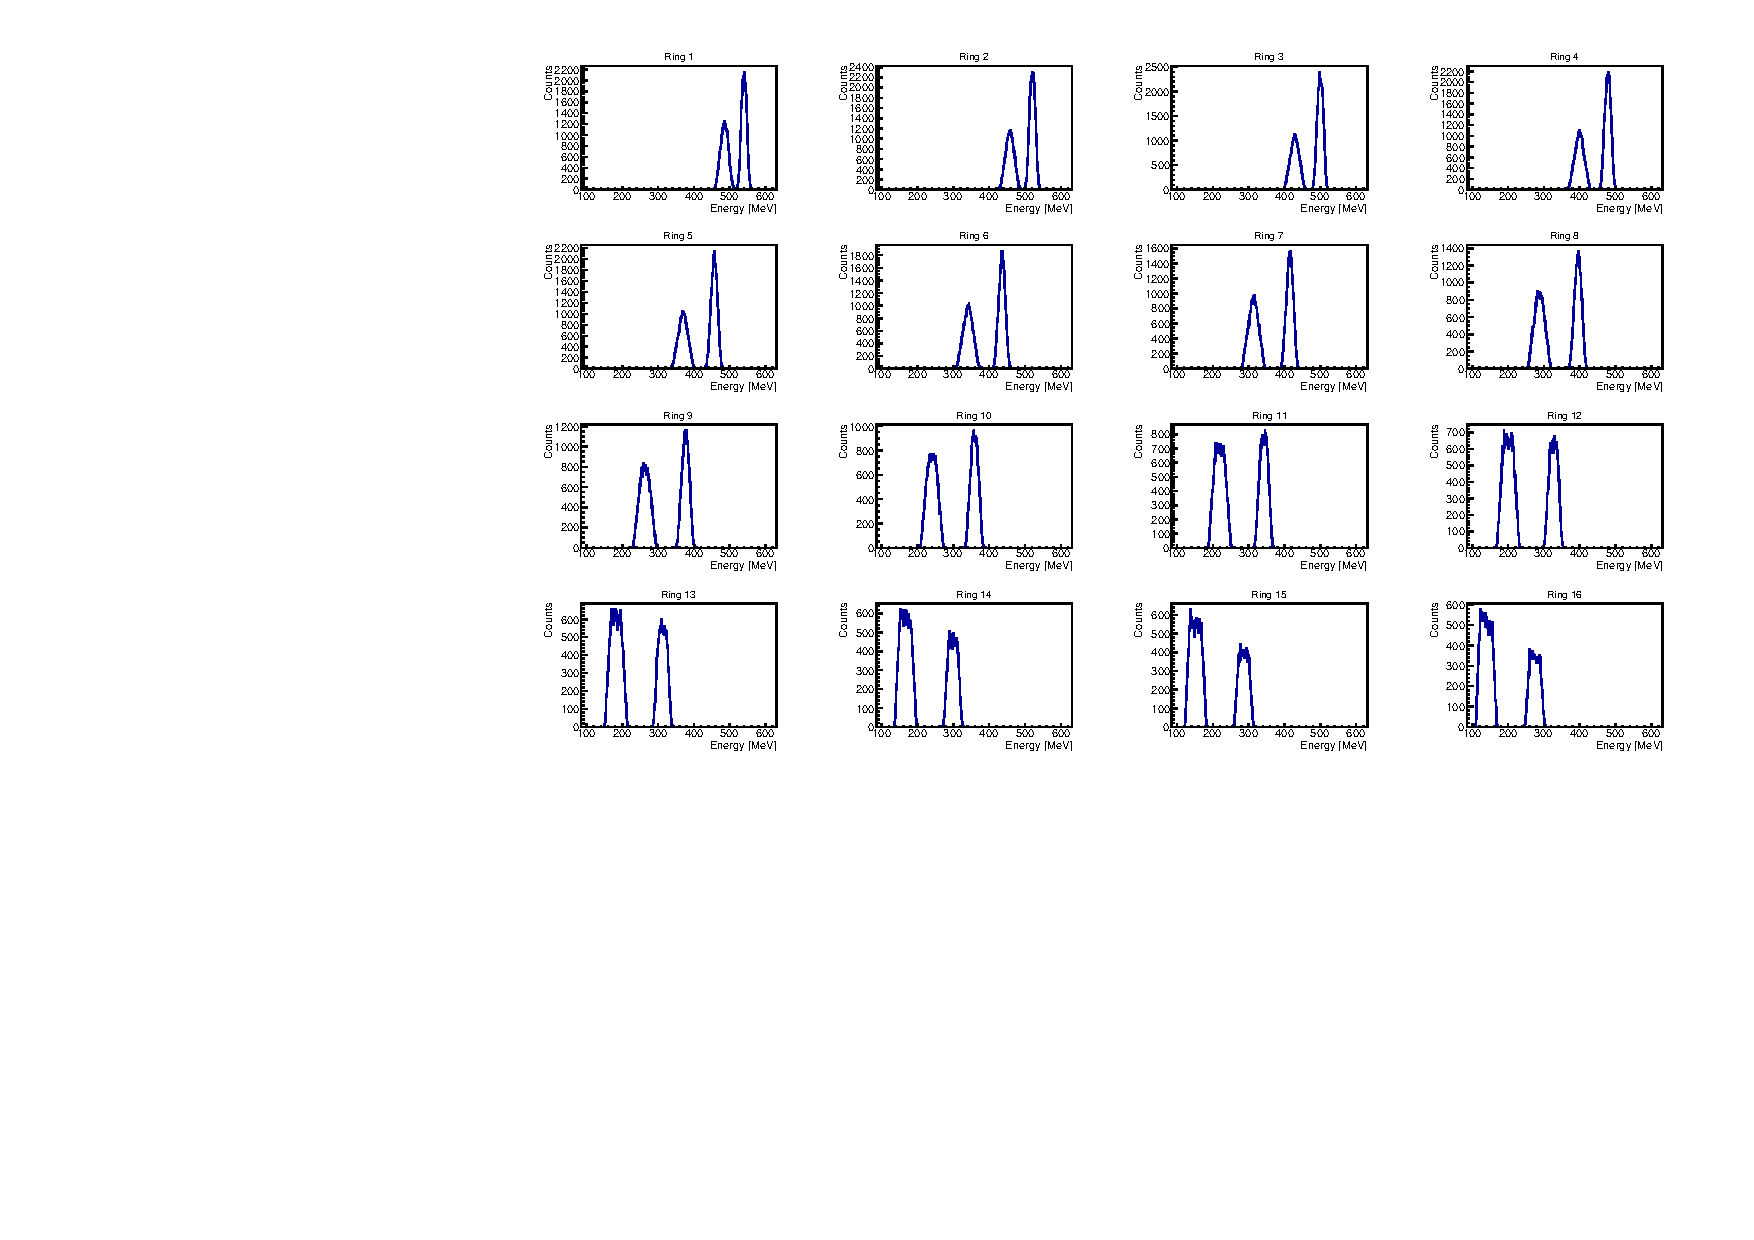
\includepdf[pages={-}, angle=270]{../Plots/simulation/cd_sim_all.pdf}


\end{appendices}



%\bibliographystyle{unsrtnat}
\bibliographystyle{mybibstyle} %my own bibstyle to set first names to one letter + unsrtnat

\bibliography{/Users/trondwj/GitHub/MasterThesis/Thesis/Mendeley/test.bib,/Users/trondwj/GitHub/MasterThesis/Thesis/References/web_references.bib}


\end{document}